\documentclass[12pt, letterpaper]{article}
\usepackage{helvet}
\usepackage{geometry}
\usepackage{amsmath}
\usepackage{graphicx}

\graphicspath{ {./images/} }
\geometry{margin=0.75in}
\renewcommand{\familydefault}{\sfdefault}

\title{Physics III: Chapter 34 - Notes from the Reading}
\author{Jake Kratt}

\begin{document}
\maketitle

This chapter continues from the electromagnetic waves discussed in Chapter 33. For the next few chapters on optics, we'll be focusing on light as an electromagnetic wave. This chapter will begin by discussing the nature of light and early methods for measuring the speed of light. Next, we'll be looking at the phenomena of geometric optics: reflection from a surface and refraction as light crosses the boundary between two media. After all of that, we'll take a look at what's called total internal refraction, which is the basis of operation for things like fiber optic cables. All of this will give us a decent background of knowledge going into Chapter 35, which will take a look at how light interacts with mirrors and lenses.

\section*{34.1. The Nature of Light}
(Disclaimer: this is a bunch of history, so if you're looking for equations, you gotta skip ahead a little.) 
\begin{itemize}
    \item Before the 19th century, light was just viewed as a stream of particles that was either emitted by an object (like a flashlight or a candle or THE SUN), or emanated from the eyes of the viewer. Basically, Isaac Newton held to the idea that particles emitted from a light source and that these particles simulated our sense of sight. He was mostly correct, but this idea is still incomplete.
    \item This idea was fine for a while, but another theory arose during his lifetime, one that argued that light might actually be some sort of wave motion. In 1678, Dutch physicist Christiaan Huygens showed that a wave model of light could also explain how light reflects of surfaces and refracts through things like glass or water.
    \item Fast-forwarding a bit to 1801, Thomas Young gave the first clear experimental demonstration of the wave nature of light. He showed that under the right conditions, light rays interfere with each other according to the waves in interference model, just like mechanical waves. This idea could've never been reached with the particle model of light, because the idea that two particles could come together and cancel each other out was inconceivable. Throughout the 19th century, the light-wave model became the dominant idea, and one of the most important developments in this model was from the work of Maxwell, who asserted that light was a form of high-frequency electromagnetic wave.
    \item However, in the 20th century, scientists found out that Newton was also right! Light also bears a particle nature under certain conditions. For this chapter, we'll just be looking at the wave nature of light. 
    \item For a while, it was effectively impossible to examine the speed of light in any laboratory. While there were efforts, many of them, like those of Galileo, who had hypothesized that by placing two lamps approximately 10km apart from each other, one would shutter one lantern for the other to shutter their lantern when they see the change, were inconclusive. However, there were a couple that were successful, and we'll be taking a look at those.
\end{itemize}

\subsection*{Roemer's Method}

\begin{itemize}
    \item In 1675, Danish astronomer Ole Roemer made observations that led to the first conclusive estimate of the speed of light. His technique involved observing Io, one of Jupiter's moons. Io takes about 42.5 hours to orbit Jupiter.
    \item An observer using Io as a basis for a clock would expect it to consistently orbit around Jupiter in 42.5 hours. However, over the course of a year, Roemer noticed that the orbital period varied. He found that eclipses of Io were later than expected when the Earth was at position $E_{1}$ on the figure, and was earlier when at position $E_{2}$ on the figure.
    \item Roemer concluded that this had to be due to the speed that light travels.
\end{itemize}

\large \textbf{Figure 34.1}

\begin{center}
    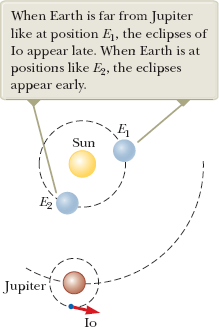
\includegraphics{roemer.png}
\end{center}

\begin{itemize}
    \item \normalsize Using Roemer's data, Huygens estimated the lower limit of the speed of light to be $2.3 \times 10^{8}m/s$. This experiment showed that light has a finite speed, a historical discovery.
\end{itemize}

\subsection*{Fizeau's Method}

\section*{34.2. The Ray Approximation in Ray Optics}
\normalsize\textbf{Ray optics} (sometimes called geometric optics) involves studying how light propagates. Ray optics assumes that light travels in a fixed direction, in a straight line, and it \textbf{stays in the same direction} if a medium it passes through is uniform until it meets a surface. At which point, it'll change directions. 

\subsection*{Figure 34.3}
\begin{center}
    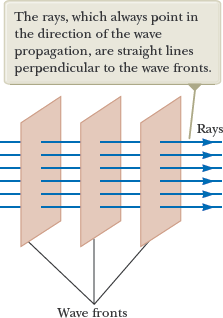
\includegraphics{34.3.png}
\end{center}
If the wave 

\subsection*{Figure 34.4}
\begin{center}
    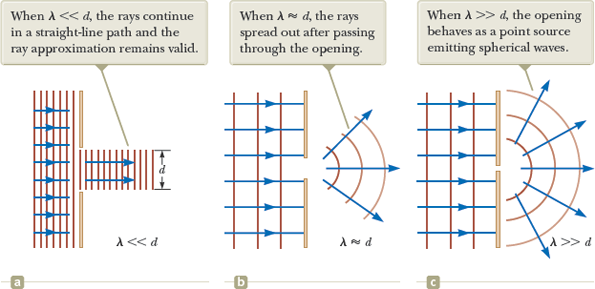
\includegraphics{34.4.png}
\end{center}

\section*{34.3. Analysis Model: Wave Under Reflection}
Here are some key terms for reflection:
\begin{itemize}
    \item \textbf{Specular reflection}: reflection of light from a smooth surface
    \item \textbf{Diffuse reflection}: reflection from any rough surface
\end{itemize}

\subsection*{Figure 34.5}
Schematic representation of (a) specular reflection, where reflected rays are parallel to one another, and (b) diffuse reflection, where light is traveling in a bunch of random directions, and then you have photographs to correspond with each.
\begin{center}
    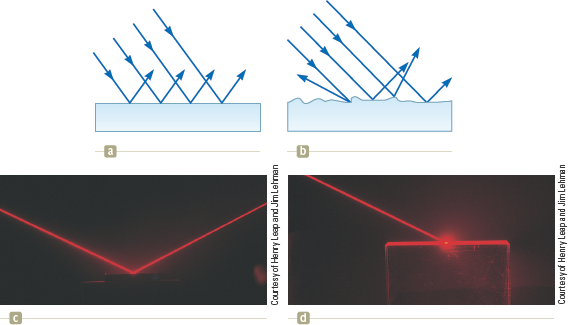
\includegraphics{34.5.png}
\end{center}
\begin{itemize}
    \item \textbf{The law of reflection} - the angle of reflection is equal to the angle of incidence: $\theta'_{1}=\theta_{1}$
    \item Because the reflection of waves is so common, there's a visual model for this.
\end{itemize}

\subsection*{Figure 34.6}
\begin{center}
    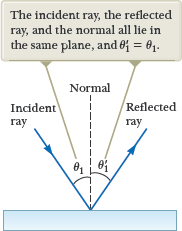
\includegraphics{34.6.png}
\end{center}

\section*{34.4. Analysis Model: Wave Under Refraction}

\section*{34.5. Huygens' Principle}

\subsection*{Huygens' Principle Applied to Reflection and Refraction}

\section*{34.6. Dispersion}

\section*{34.7. Total Internal Reflection}

\subsection*{Optical Fibers}

\end{document}